\documentclass[10pt]{article}
\usepackage[ngerman]{babel}
\usepackage[utf8]{inputenc}
\usepackage[T1]{fontenc}
\usepackage{amsmath}
\usepackage{amsfonts}
\usepackage{amssymb}
\usepackage[version=4]{mhchem}
\usepackage{stmaryrd}
\usepackage{graphicx}
\usepackage[export]{adjustbox}
\graphicspath{ {./images/} }
\usepackage{bbold}

\title{Hauptprüfung Abiturprüfung 2023 - Leistungsfach }

\author{Alexander Schwarz\\
www.mathe-aufgaben.com}
\date{}


\begin{document}
\maketitle
 Baden-Württemberg

\section*{Aufgabe B1}
Auf einem ebenen, horizontalen Gelände steht ein 15 m hoher Mast, an dem drei rechteckige Werbeflächen befestigt sind. In der Abbildung 1 ist eine der Werbeflächen grau dargestellt.\\
Der Mast ist zylinderförmig und hat einen Durchmesser von 80 cm ; er verläuft ebenso wie die seitlichen Kanten der Werbefläche vertikal.

In einem Koordinatensystem wird das Gelände durch die $\mathrm{x}_{1} \mathrm{x}_{2}$ - Ebene beschrieben; eine Längeneinheit im Koordinatensystem entspricht 1 m in der Wirklichkeit.\\
Der Mittelpunkt der Grundfläche des Masts wird durch den Koordinatenursprung dargestellt.\\
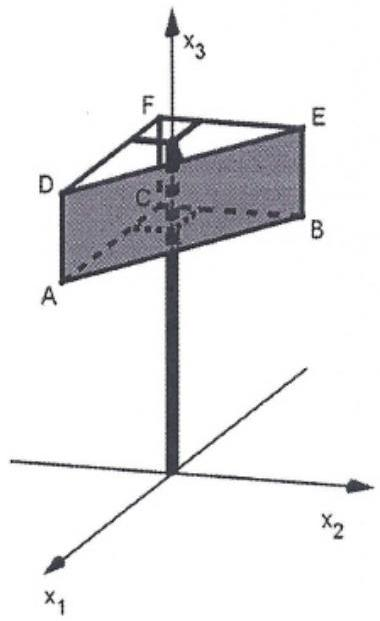
\includegraphics[max width=\textwidth, center]{2025_04_24_8932b081615df7225b10g-2(1)}

Abb. 1 Die Punkte $\mathrm{A}(5|-2| 11), \mathrm{E}(-2|5| 15)$ und $\mathrm{F}(-2|-2| 15)$ stellen Eckpunkte der Werbeflächen dar.\\
a) Bestimmen Sie den Flächeninhalt der grau dargestellten Werbefläche.

Prüfen Sie, ob die beiden anderen Werbeflächen einen rechten Winkel einschließen.\\
b) Die grau dargestellte Werbefläche liegt im Modell in einer Ebene, deren Gleichung in der Form $\mathrm{a} \cdot \mathrm{x}_{1}+\mathrm{a} \cdot \mathrm{x}_{2}=\mathrm{b}$ dargestellt werden kann. Ermitteln Sie passende Werte von a und b .\\
c) Begründen Sie, dass der Abstand der grau dargestellten Werbefläche zum Mast mit dem Abstand des Mittelpunkts der oberen Kante dieser Werbefläche zum Mast übereinstimmt.

Auf dem Gelände befindet sich ein Sportplatz. Von dort aus blickt ein Kind zur grau dargestellten Werbefläche. Die Sicht des Kindes wird durch eine Mauer eingeschränkt. Die obere Kante der Mauer wird im Modell durch die Strecke zwischen den Punkten P(20|-5|3) und Q (20|25|3) dargestellt. Der Punkt, von dem der Blick des Kindes ausgeht, wird durch K(24|15|1) beschrieben. Das Kind kann denjenigen Teil der Werbefläche, der durch das Dreieck GBH mit\\
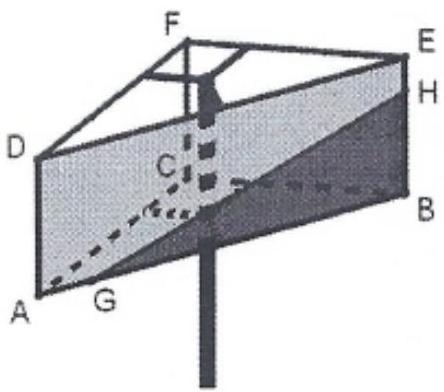
\includegraphics[max width=\textwidth, center]{2025_04_24_8932b081615df7225b10g-2}

Abb. 2 $\mathrm{G}(4|-1| 11)$ dargestellt wird, nicht sehen (siehe Abbildung 2).\\
d) Eine Sichtlinie verläuft im Modell von K zu G. Berechnen Sie die Größe des Winkels dieser Sichtlinie gegenüber der Horizontalen.\\
Beschreiben Sie, wie man die Koordinaten von H rechnerisch bestimmen könnte.\\
e) Auf dem Sportplatz wird ein Fußball geschossen. Die Flugbahn des Balls wird im Modell durch Punkte der Form $R_{t}\left(32-8 t|5|-5 t^{2}+6,5 t+0,3\right)$ mit $t \in \mathbb{R}^{+}$ beschrieben. Dabei ist t die seit dem Schuss vergangene Zeit in Sekunden. Der Ball bewegt sich im Modell in der Ebene L. Beschreiben Sie die besondere Lage von L im Koordinatensystem und geben Sie eine Gleichung dieser Ebene an.

\section*{Lösungen}
\section*{Aufgabe B1}
a) Bestimmen Sie den Flächeninhalt der grau dargestellten Werbefläche.

Zunächst benötigt man die Koordinaten von Punkt B.\\
$B$ befindet sich direkt unterhalb von $E$ und hat denselben $x_{3}$-Wert wie $A$.\\
Koordinaten: B(-2|5|11)\\
Die Werbefläche ist ein Rechteck.\\
Flächeninhalt des Rechtecks: $|\overrightarrow{\mathrm{AB}}| \cdot|\overrightarrow{\mathrm{BE}}|=\left|\left(\begin{array}{c}-7 \\ 7 \\ 0\end{array}\right)\right| \cdot 4=\sqrt{98} \cdot 4 \approx 39,6 \mathrm{~m}^{2}$\\
Prüfen Sie, ob die beiden anderen Werbeflächen einen rechten Winkel einschließen.

Die beiden anderen Werbeflächen bilden einen rechten Winkel, wenn gilt:\\
$\overrightarrow{F E} \cdot \overrightarrow{F D}=0$.\\
Der Punkt D hat die Koordinaten $\mathrm{D}(5|-2| 15)$.\\
$\overrightarrow{\mathrm{FE}} \cdot \overrightarrow{\mathrm{FD}}=\left(\begin{array}{l}0 \\ 7 \\ 0\end{array}\right) \cdot\left(\begin{array}{l}7 \\ 0 \\ 0\end{array}\right)=0$\\
Das heißt, die beiden anderen Seitenflächen schließen einen rechten Winkel ein.\\
b) Ermitteln Sie passende Werte von a und b.

Die Werte von a und b können durch das Einsetzen des Punktes $A(5|-2| 11)$ in die Ebenengleichung ermittelt werden:\\
$a \cdot 5+a \cdot(-2)=b \Leftrightarrow 3 a=b$\\
Wählt man für $a=1$ ergibt sich für $b=3$.\\
Ebenengleichung: $x_{1}+x_{2}=3$\\
Hinweis:\\
Da die Koordinatengleichung einer Ebene nicht eindeutig ist (sie kann beliebig vervielfacht werden), gibt es keine eindeutige Lösung für $a$ und $b$.

Man hätte beispielsweise auch für $a=2$ wählen können, dann wäre $b=6$ gewesen. Ebenengleichung: $2 x_{1}+2 x_{2}=6$\\
c) Begründen Sie, dass der Abstand der grau dargestellten Werbefläche zum Mast mit dem Abstand des Mittelpunkts der oberen Kante dieser Werbefläche zum Mast übereinstimmt.\\
1.Möglichkeit: Rechnerische Begründung

Abstand der Ebene $\mathrm{H}: \mathrm{x}_{1}+\mathrm{x}_{2}=3$ zum Mast:\\
Da der Mast ein Zylinder ist, der symmetrisch um die $x_{3}$-Achse liegt, wird zunächst der Abstand der Ebene zum Endpunkt des Mastes R(0|0|15) bestimmt:

HNF von $H: \frac{x_{1}+x_{2}-3}{\sqrt{2}}=0$\\
Abstand von $R$ zu $E: d(R, H)=\frac{|-3|}{\sqrt{2}}=\frac{3}{\sqrt{2}} \mathrm{~m}$\\
Der Abstand von H zum Zylinderrand beträgt damit $\frac{3}{\sqrt{2}}-0,4 \mathrm{~m}$.\\
Der Mittelpunkt der oberen Kante zwischen $\mathrm{D}(5|-2| 15)$ und $\mathrm{E}(-2|5| 15)$ lautet M(1,5|1,5|15).

Der Abstand von Punkt M zur $x_{3}$-Achse entspricht dem Abstand von $M$ zum Punkt R(0|0|15), da beide Punkte auf gleicher Höhe sind und die Strecke $\overline{\mathrm{RM}}$ senkrecht auf der $\mathrm{x}_{3}$-Achse steht.\\
$|\overrightarrow{R M}|=\left|\left(\begin{array}{c}1,5 \\ 1,5 \\ 0\end{array}\right)\right|=\sqrt{1,5^{2}+1,5^{2}}=\sqrt{4,5}=\frac{3}{\sqrt{2}}$\\
Der Abstand von $R$ zum Zylinderrand beträgt damit $\frac{3}{\sqrt{2}}-0,4 \mathrm{~m}$ und stimmt mit dem Abstand der Werbefläche zum Zylinderrand überein.

2.Möglichkeit: Begründung per Argumentation
Die $\mathrm{x}_{3}$-Achse ist die Symmetrieachse des zylinderförmigen Mastes.\\
Das Dreieck mit den Eckpunkte D, E und $\mathrm{R}(0|0| 15)$ (Endpunkt des Mastes) ist außerdem gleichschenklig, da $|\overrightarrow{D R}|=|\overrightarrow{E R}|=\sqrt{25+4}=\sqrt{29}$.\\
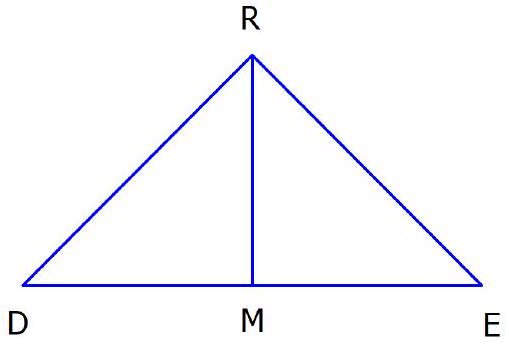
\includegraphics[max width=\textwidth, center]{2025_04_24_8932b081615df7225b10g-5}

Daher hat der Mittelpunkt M der Strecke $\overline{\mathrm{DE}}$ den kürzesten Abstand von R .\\
Da die Werbefläche parallel zur $\mathrm{x}_{3}$-Achse verläuft, gibt es auch keinen anderen Punkt auf der Werbefläche, der einen kleineren Abstand zu dem Mast hat.\\
d) Berechnen Sie die Größe des Winkels dieser Sichtlinie gegenüber der Horizontalen.

Es gilt $\overrightarrow{\mathrm{GK}}=\left(\begin{array}{c}20 \\ 16 \\ -10\end{array}\right)$\\
Gesucht ist der Winkel zwischen der Geraden mit dem Richtungsvektor $\overrightarrow{\text { GK }}$ und der $x_{1} x_{2}$-Ebene mit dem Normalenvektor $\vec{n}=\left(\begin{array}{l}0 \\ 0 \\ 1\end{array}\right)$.\\
$\sin \alpha=\frac{\left(\left.\left(\begin{array}{c}20 \\ 16 \\ -10\end{array}\right) \cdot\left(\begin{array}{l}0 \\ 0 \\ 1\end{array}\right) \right\rvert\,\right.}{\sqrt{400+256+100} \cdot \sqrt{1}}=\frac{10}{\sqrt{756}} \quad \Rightarrow \alpha \approx 21,3^{\circ}$

Beschreiben Sie, wie man die Koordinaten von H rechnerisch bestimmen könnte.\\
1.) Da der Punkt H auf der Geraden durch B und E liegt wird die Gleichung der Gerade h durch die Punkte B und E aufgestellt.\\
2.) Da das Kind vom Punkt $K$ aus in unendlich vielen Richtungen direkt über die Mauerlinie schauen kann, liegen die optischen Strahlen in der Ebene Z, die durch die Punkte K, P und Q verlaufen.\\
3.) Der gesuchte Punkt H ist der Schnittpunkt der Ebene $Z$ und der Gerade h.\\
e) Beschreiben Sie die besondere Lage von L im Koordinatensystem und geben Sie eine Gleichung dieser Ebene an.

Aufgrund der Koordinaten von $R_{t}\left(32-8 t|5|-5 t^{2}+6,5 t+0,3\right)$ erkennt man, dass die $x_{2}$-Koordinate konstant ist.\\
Damit liegt die Ebene $L$ parallel zur $x_{1} x_{3}$-Ebene: $L$ : $x_{2}=5$.\\
Untersuchen Sie, ob der Ball die Mauer trifft, bevor er den Boden berührt.\\
Aufgrund der Koordinaten von $P$ und $Q$ und da die Mauer senkrecht zum Boden steht erkennt man, dass der Aufprallpunkt des Balles die $\mathrm{X}_{1}$-Koordinate 20 haben muss.

Bedingung: $32-8 t=20 \Rightarrow t=1,5$\\
Einsetzen von $t=1,5$ in den allgemeinen Punkt ergibt $R_{1,5}(20|5|-1,2)$.\\
Da die $x_{3}$-Koordinate negativ ist, trifft der Ball die Mauer nicht, bevor er den Boden berührt.


\end{document}